%%%%%%%%%%%%%%%%%%%%%%%%%%%%%%%%%%%%%%%%%%%%%%%
\chapter{How Might Online Systems Support Citizen-led Knowledge Work}

\begin{quote}
\emph{This dissertation explores how }
\end{quote}
\vspace{0.25in}

Todo- text here

\section{Opportunity: Harnessing humanity\textquotesingle s collective efforts accomplishes great goals}
Luis von Ahn said people can build eiffel towers but people are barely able to build those eiffel towers - -why? But why build eiffel towers for other people?

poor signal-to-noise from crowds due to lack of training; inefficient collaboration without careful attention; and poor results (or no results at all) unless experts lead. To address these concerns, my work introduces and evaluates peer production architectures and procedural learning.

\subsection{People have complementary knowledge in comparison to experts and are uninfected by expert biases}
--drawn from lived experience
-- individually and collectively

Sometimes, having a different background than experts can
be beneficial. Shared knowledge is great when it’s right, but
blocks progress when wrong. When false assumptions limit
experts, at least some novices are likely to be “uninfected”.
For example, GalaxyZoo volunteers discovered ‘green pea’
galaxies overlooked by scientists who mistakenly assumed
the green hue was merely an imaging artifact [54]. 

\subsection{Learning resources proliferate and people learn from personal interest/hobby but it's not directly linked to their personal thing}
Creative, open-ended work has rich pedagogical value.
Online work, like online learning, requires appropriate
scaffoldings, such as rubrics [12,41], decision trees [43,57],
tutorials [6], and quick expert guidance [23]. Similar to
general critique of pure discovery learning [47], simply
asking participants to “figure it out” would be poor pedagogy. Hence, Gut Instinct introduces a guided discovery
learning approach as Mayer advocates: expert-curated
learning materials help participants start, with discovery
following. Recruiting learners as citizen scientists offers a
Problem-based Learning experience with context and motivation for the material students learn [50]. In principle,
these real-world problems also provide a yardstick for
measuring learning. 

\subsection{Second-order effect: People are connected online and collectively have access to many resources}
In a large distributed community, there’s often
someone who happens to have important relevant
knowledge, usually drawing on a relevant but distant domain. Such distributed efforts are a type of lead-user innovation [31]. Having many people work on the same problem increases the odds that one will break through. Drawing
on secondary expertise as inspiration can be an important
agent of creativity because almost by definition, the combination is rare [10]. Open \& crowd innovation builds up on
contributions by diverse online participants, and a ‘bubbling
up’ process for strong ideas [56].

\section{Challenge: People don't know how to perform expert work}
Problem Dimensions


\subsection{People lack the expertise to make situationally-appropriate choices and people aren\textquotesingle t trained in these things}
-- people dont know how to use their knowledge
Why is this complex: requires making many choices

The
converse also holds, and much more often: novices are also
“uninfected” by all the knowledge that enables experts to
innovate.

\subsection{People lack a professional network to improve their work}


\subsection{People lack the time/remuneration/resources to learn new things and implement them in their lives}
nnk

********
Further, recreating expert work context, process, and outcomes can alter and reduce the value of novice contributions.

My research raises the question: how can global communities create knowledge that meets their goals without waiting for experts to lead? My research prototypes collective systems for large-scale problems.

********
\section{Thesis: Procedural Support for Roles}

Many people have strong personal motivations and contextual insights. To create knowledge,
they need mental scaffolds for organizing complex work, domain knowledge to compose and
execute the steps, and ways to ask for help. Professional scientists benefit from conceptual
knowledge, professional training, pre-existing organizational structure for collaboration, and direct access to resources. Currently, citizens lack these resources.

Building on these new participation channels, we suggest that democratizing experimentation may
also expand the gamut of scientific knowledge. People have questions about their health, but lack
the expertise and resources to scientifically investigate them. How might online systems support
more complex activities that leverage the creativity and diversity of a global community?

This dissertation explores challenges people face xxxxxxx. Underlying these investigations is the thesis:

//this is where you introduce the taxonomy 
//provide fig here from the research statement 

"My thesis statement is"
\begin{quote}
\emph{Integrating conceptual learning with task-specific scaffolding enables personally meaningful \& useful scientific work}
\end{quote}


%%%%%%%%%%%
\section{Contributions}
\begin{figure}[t!] 
  \centering
    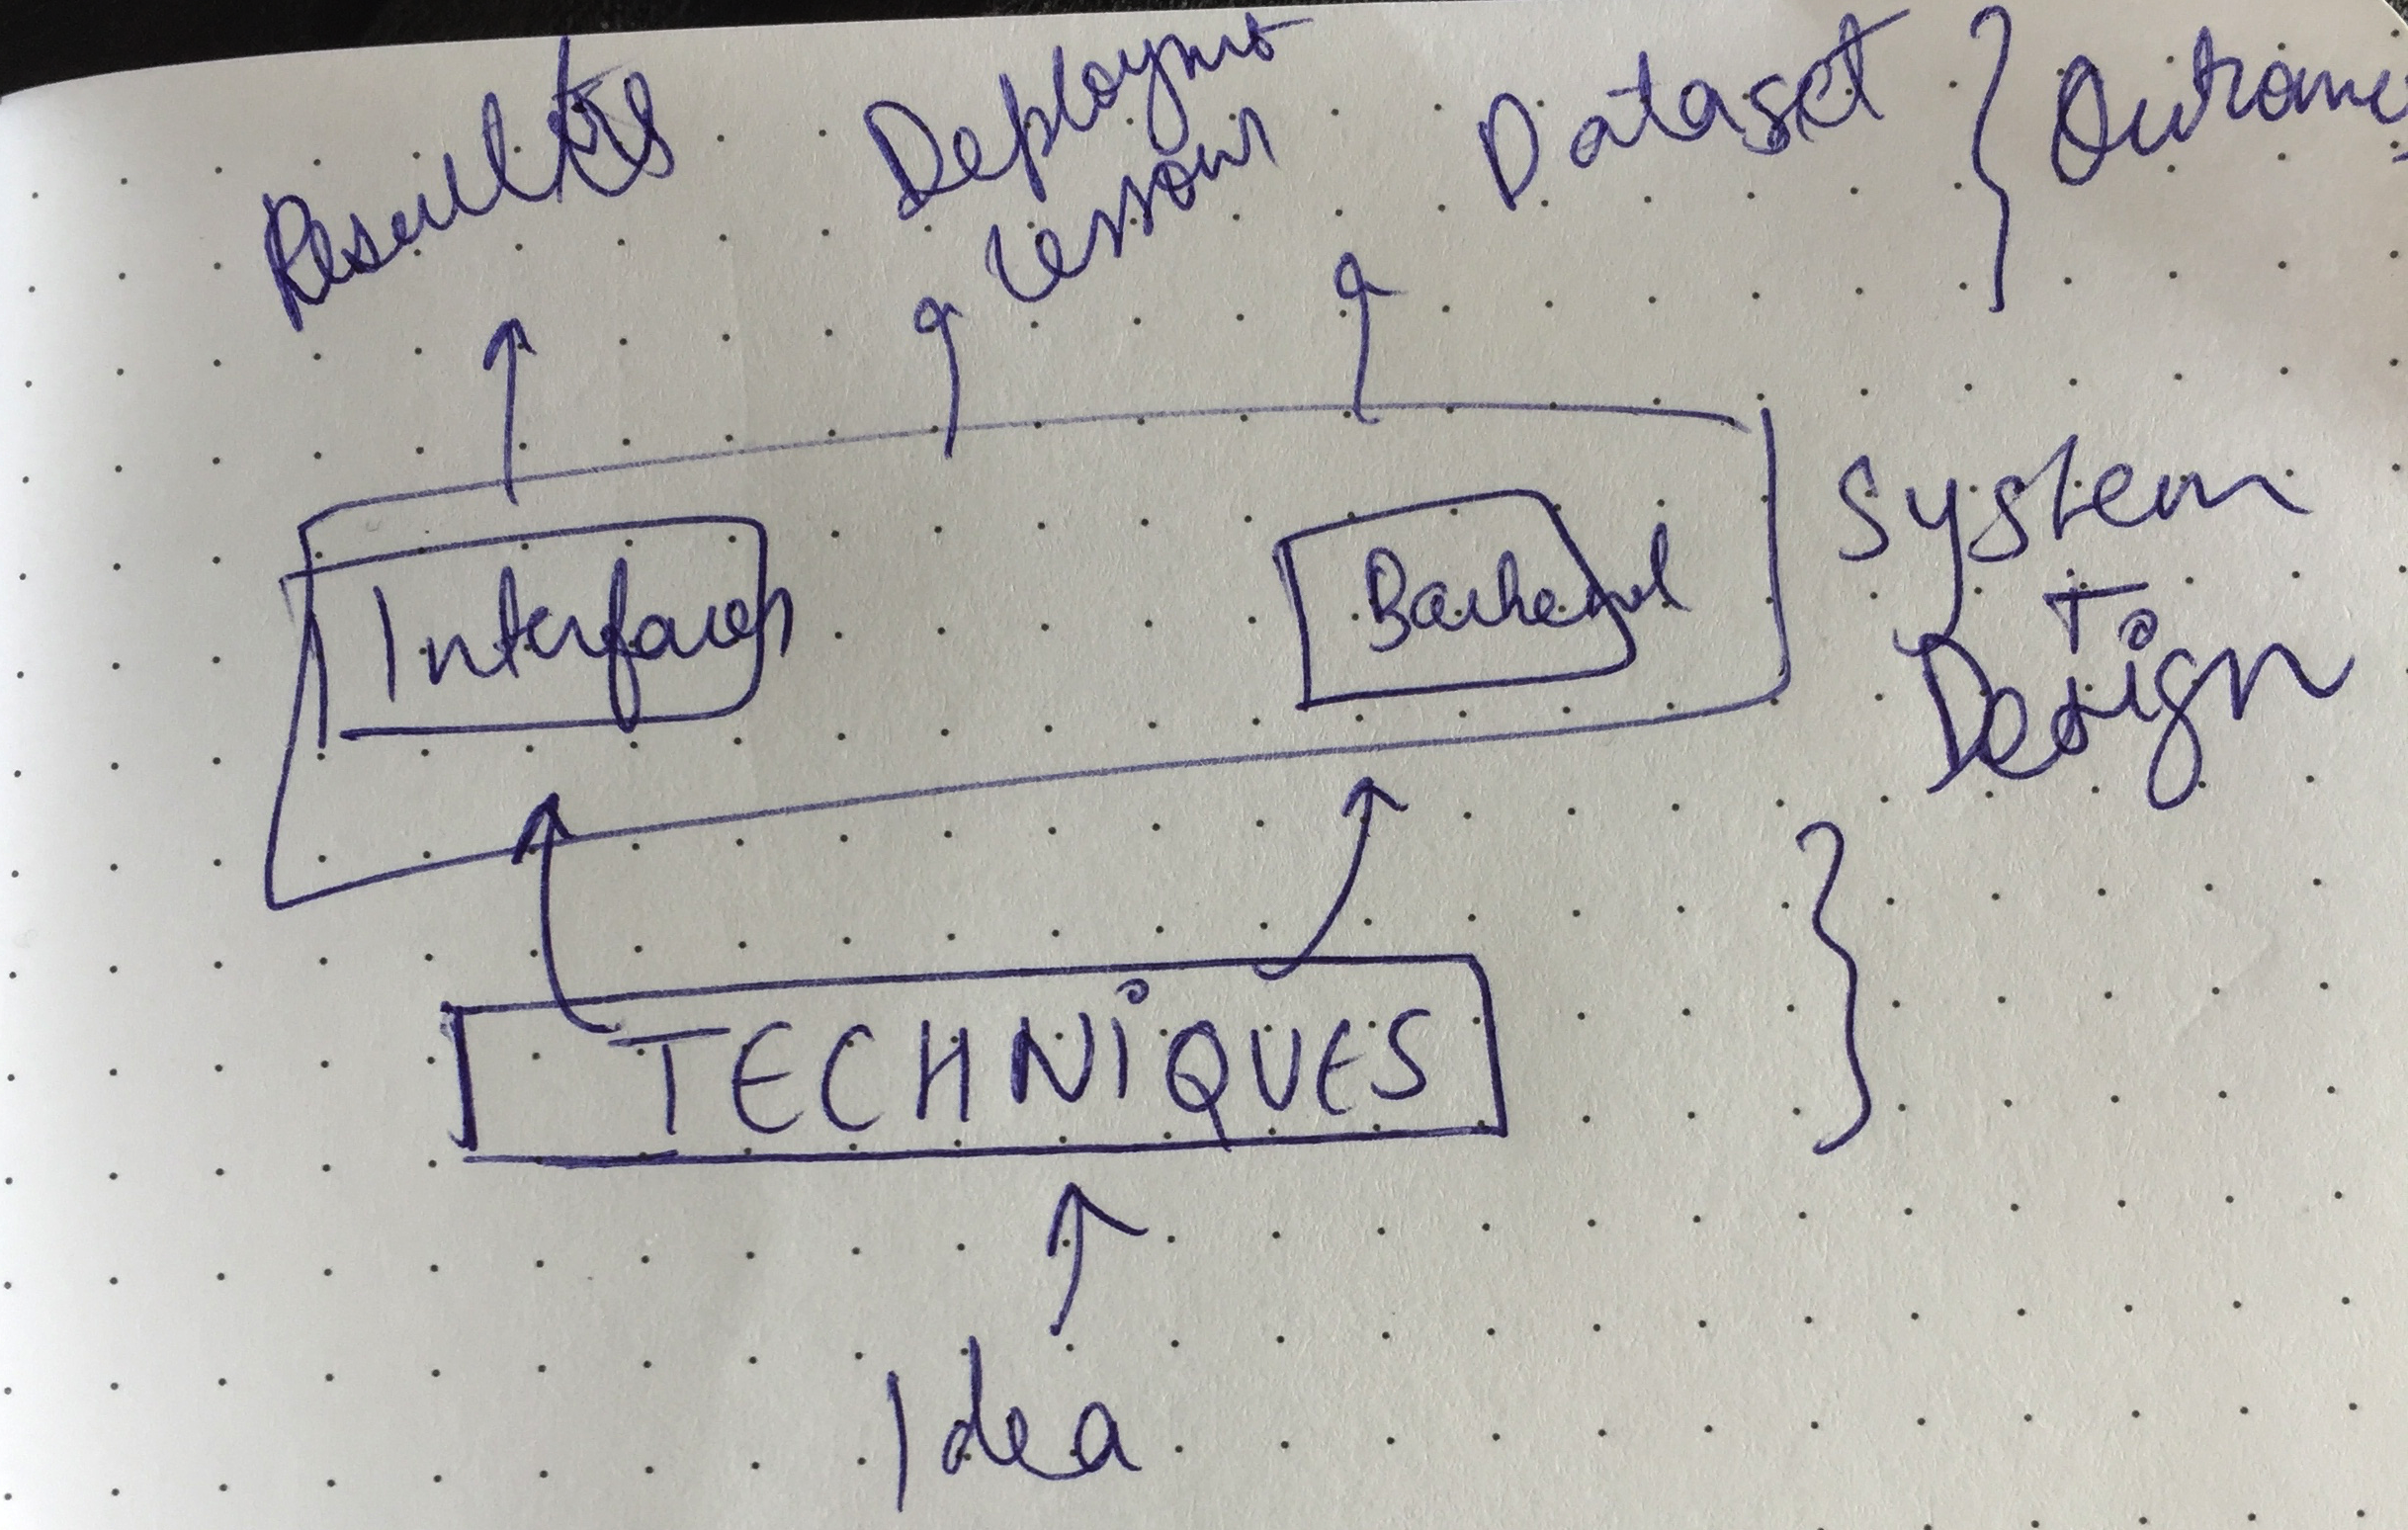
\includegraphics[width=1.0\textwidth]{figures/img/intro/1-contributions}
  \caption[Contributions of this dissertation]
{Contributions of this dissertation including empirical results theoretical perspectives/techniques, real-world systems, and multiple outcomes}
  \label{fig:contributions}
\end{figure}

This dissertation\textquotesingle makes two assumptions: 1) most people have an amazing breadth and depth of ideas , and 2) they lack the expertise to implement these ideas. Consequently, both people and the world lives in a severely sub-optimal space.

Two major issues in enabling complex work on the internet are (diversity and scale?) quality of individual contribution and the overall management of contributions.  We desire social computing techniques that reliably enable a wide variety of people to contrinute more than they naturally could and that manage the dependencies among a large set of tasks.

This dissertation\textquotesingle s primary contribution is the idea of intergrating learning in social computing to enable groups of novices to perform complex, creative task. To realize this idea, this dissertation makes three types of contributions: theoretical perspectives/techniques, real-world systems, and outcomes including empirical results, systems lessons, and dataset (Figure \ref{fig:contributions}). The techniques make the idea concrete; the system operationalizes the techniques and makes them work; and the outcomes discuss the successes and failures of our approach.

%todo - need terms for these


\subsection{Idea: Dual-objective online learning systems}
Dual objective systems have been around  a while. Commercial systems developed by Facebook and Google typically serve two purposes: provide a service to people (email, photos) and collect data; such data is used to train and improve Machine Learning algorithms, sold to third parties, and used for in-house advertising plans. While people receive the benefits of such technologies, it happens automagically.They don\textquotesingle 't learn anything.

My thesis proposes another future for dual objective systems --one where people perform work that is useful for others and the platform, but they also meet their needs. 
%add the system and people-led learning bits to social computing / crowdsourcing parts

\subsection{Theoretical: Techniques and Framework}
Improving the quality of work requires improvements at two levels: both the depth of work done per individual and the amount of work done overall. The former require better learning tools and the latter requires better collaboration tools and dependency management. 

Theoretical contributions include 1) principles to integrate learning in social computing, 2) User nterfaces and system design for efficient implementation", and 3) a characterization of the classes of activities that can work with this model.

\begin{itemize}
% come up with principles myself
\item Principles to integrate learning in social computing 
There are two kinds of learning: conceptual (declarative) and procedural. A large part of current education is about conceptual learning, where people learn what something is, learn about its features. Typically, such learning is tested with test questions. In contrast, procedural learning teaches the {\it how} of things. How do you do x, y, or z.  Concpetual learning is useful when xxx while procedural learning is more useful when yyy.

%figure about conceptual and procedural learning 

For useful contribution to complex work, people need to have a good working model of both the concepts and procedures for a thing. How does my dissertation deal with this?
1. reify conceptual bits in the software itself or provide via video //
2. Drawing from learning psychology and not attention psychology 
-- see the ethical engineering award thing
3. 

The efficacy of these techniques is borne out over multiple deployments. 

\item  Principles to decompose Complex work to f(people, community, \& machines)
% figure -- def needs one -- based on strengths and weaknesses

Social computing relies on carefully designing the affordances, support, and system to enable different users for different needs.

1. The individual, a group, and groups of machines possess complementary strengths. \\
Individual: creative, lived experience gives ideas, personal context, creative, willing to push through \\
community: lesser motivation but willing to help (diff roles to contribute), another set of eyes, diverse ideas --> check biases \\
machines: consistent implementation, reduces biases
(see slide deck)

2. Think of complex work as simpler tasks where the system manages the interdependencies

proof: success of the experimentation platform

\end{itemize}

All these techniques have been put in systems as interfaces, intelligent backends, and so on... \\
//present a stack of things

\subsection{System Design (including Interfaces)}
%%"Furthermore, adding location information to photo collections is by itself insufficient for scenevisualization: we also need intuitive, interactive interfaces for exploring these scenes. There are several challenges faced in the design of such interfaces. First, unlike with Google Street View, where photos are taken at regular intervals, personal or Internet collections are typically an unstructured soup of photos. Nevertheless, the navigation controls should still be intuitive and exhibit regularity. Second, such controls should make it easy to find and explore the interesting parts of a scene, particularly for tourist sites."


Furthermore, providing techniques is not enough. 

The techniques described above need to be implemented in ways that are easy to understand, access, and use for most people. This happens by baking these in the user interface (which is the direct thing people interact with) and by building a backend that is based on the principles of x, y, and z.

\subsubsection{User Interfaces}
\begin{itemize}
\item UIs that implement learning ( conceptual + procedural)
\item UIs for focused collaboration  
\end{itemize}

\subsubsection{System design}

\begin{itemize}
\item system-led learning vs people-led
\item Backend that manages the task dependency, and transparency among users
--- finite state machine (history of...)
--- drawing from parser, compiler + lex/yacc format for this state machine for complex tasks ideas
\item  db optimizations
\end{itemize}

state diagram — the edges represent what people need to do 

\subsubsection{Roles Support via Just-in-time Skill Acquisition}
 People take different roles
--write up form galileo


%%%%%%%%%%%%%
\subsection{Outcomes}
\subsubsection{Empirical Results from Real-world Deployment}
expertise: limited; diversity: different countries; scale: some

\subsubsection{Lessons}
\begin{itemize}
\item improved methods to test usability of my systems and techniques -- via multiple deployments
\item xxx
\end{itemize}

\subsubsection{Dataset}
1. repo of hypotheses with rating
2. repo of experimental designs
3. ...

\section{Impact}
 \subsection{Used by communities}
 \subsection{Talks in the Research community and other communities}
 \subsection{Taught in classes}


\section{Dissertation Roadmap}

%%%%%%%%%%%%%%%%%%%%%%%%%%%%%%%%%%%%%%%%%%%%%%%%%%%%%%%%%%%%%%%%%%
%todo- “we” refers to the set of authors…  -- see arvind


"double quotes"

